\documentclass[../VD.tex]{subfiles}

\externaldocument{../VD}

\begin{document}

\setcounter{chapter}{2}
\chapter{Subvariedades}\label{chap:subvd}

\section{Introducción}
\label{sec:subvd-intro}

\begin{definition}[name={subvariedad},label={def:subvd}]
  Dada una \(m\)-variedad \(M\), un subconjunto \(N \subseteq M\) se dice que es
  \emph{\(n\)-subvariedad} de \(M\) (\(n \leq m\)) si para todo \(p \in M\)
  existe una carta \((U,\varphi)\) de \(M\) con \(p \in U\) y tal que
  \begin{equation}
    \label{eq:subvd-cond}
    varphi(U) \cap \RealSet^{m} = \varphi(U \cap N)
  \end{equation}

  Aquí, \(\RealSet^{n}\)
  se ve como el subespacio \(\RealSet^{n} \times \Set{0}^{m-n} \subseteq
  \RealSet^{m}\) de los puntos de \(\RealSet^{m}\) cuyas últimas \(m-n\)
  coordenadas son nulas.
\end{definition}

\begin{lemma}[label=lem:subvd-subset]
  Para todo \(A \subset U\) tenemos
  \begin{equation}
    \label{eq:lem-subvd-subset}
    \varphi(A) \cap \RealSet^{n} = \varphi(A \cap N)
  \end{equation}
\end{lemma}

\begin{proof}
  Si \(z \in \varphi(A) \cap \RealSet^{m} \subseteq \varphi(U) \cap \RealSet^{m}
  = \varphi(U \cap N)\), entonces existe \(p \in U \cap N\) con \(z =
  \varphi(p)\). Como \(z \in \varphi(A)\), \(p \in A\) y por ser inyectiva se
  tiene \(z \in \varphi(A \cap N)\).

  Si \(z \in \varphi(A \cap N) \subseteq \varphi(U \cap N) = \varphi(U) \cap
  \RealSet^{n}\), entonces \(z \in \RealSet^{n}\). Existe \(a \in A \cap N\) con
  \(\varphi(a) = z\), luego \(z \in \varphi(A) \cap \RealSet^{n}\). La otra
  contención es trivial.
\end{proof}

\begin{lemma}[label={lem:subvd-exists}]
  Para toda carta \((V,\psi)\) de \(M\) con \(p \in V\) se puede encontrar una
  carta \((W,\psi)\) con \(p \in W \subseteq V\) cumpliendo
  \eqref{eq:subvd-cond}.
\end{lemma}

\begin{proof}
  Sea \((U,\varphi)\) una carta de \(M\) cumpliendo \eqref{eq:subvd-cond}. Por
  la compatibilidad de cartas, \((W,\psi) = (U \cap V, \Restrict{\varphi}{U \cap
    V})\) es una carta de \(M\) con \(W \subseteq V\) y

  \begin{align*}
    \varphi(W) \cap \RealSet^{m}
    &= \varphi(U \cap V) \cap \RealSet^{m}\\
    &\overset{\mathclap{\eqref{eq:lem-subvd-subset}}}{=} \varphi(U \cap V \cap N)\\
    &= \varphi(W \cap N)
  \end{align*}
\end{proof}

\begin{lemma}[label={lem:subvd-vd}]
  Toda \(n\)-subvariedad \(N \subseteq M\) es una \(n\)-\nameref{def:vd}.
\end{lemma}

\begin{proof}
  Sabemos que dado \(p \in N\) existe una carta \((U_{p},\varphi_{p})\) de \(M\)
  con \(p \in U_{p}\) y \(\varphi_{p}(U_{p}) \cap \RealSet^{m} =
  \varphi_{p}(U_{p} \cap N)\).

  Entonces \((U_{p} \cap N, \Restrict{\varphi_{p}}{U_{p} \cap N}) \eqqcolon
  (W_{p}, \psi_{p})\) es un conjunto de cartas compatibles sobre \(N\).

  Notemos dos cosas:
  \begin{enumerate}
  \item \(\psi_{p}(W_{p}) = \varphi_{p}(U_{p} \cap N) = \varphi_{p}(U_{p}) \cap
    \RealSet^{n}\) es abierto de \(\RealSet^{n}\).
  \item  Si \(W_{p} \cap W_{q} \neq \emptyset\), entonces
    \begin{figure}[h]
      \centering
      \begin{tikzcd}[row sep=small]
        \mathllap{\psi_{q} \psi_{p}^{-1} \colon}
        \psi_{p}(W_{p} \cap W_{q})
        \ar[r] \ar[d,symbol={=}]
        & \psi_{q}(W_{p} \cap W_{q}) \ar[d,symbol={=}]\\
        \varphi_{p}(U_{p} \cap U_{q} \cap N) \ar[r] \ar[d, symbol={=}]
        & \varphi_{q}(U_{p} \cap U_{q} \cap N) \ar[d, symbol={=}]\\
        \mathllap{\varphi_{q} \varphi_{p}^{-1} \colon}
        \varphi_{p}(U_{p} \cap U_{q}) \cap \RealSet^{n}
        \ar[r]
        & \varphi_{q}(U_{p} \cap U_{q}) \cap \RealSet^{n}
      \end{tikzcd}
    \end{figure}

    es decir, \(\psi_{q} \psi_{p}^{-1}\) es restricción de
    \(\varphi_{q}\varphi_{p}^{-1}\) y por tanto diferenciable.
  \end{enumerate}

  Ahora aplicamos la \nameref{def:Lindelöff} a \(N \subseteq M\) y como \(N
  \subseteq \bigcup_{p \in N} U_{p}\), tenemos una cantidad numerable
  \(U_{p_{1}},\dots,U_{p_{n}},\dots\) con \(N \subseteq \bigcup_{n=1}^{\infty}
  U_{p_{n}}\), luego \(N = \bigcup_{n=1}^{\infty} W_{p_{n}}\), así que
  \(\mathcal{A} = \Set{(W_{p_{j}}, \psi_{p_{j}})}_{j \geq 1}\) es un atlas de
  \(N\).
\end{proof}

\begin{lemma}[label={lem:inclusion-inmersion}]
  La inclusión \(i \colon N \hookrightarrow M\) es una \nameref{def:inmersión}
  inyectiva.
\end{lemma}

\begin{proof}
  Obviamente \(i\) es inyectiva. Además es inmersión pues dado \(p \in N\), si
  \((U,\varphi)\) es una carta de \(M\) con \(p \in M\) cumpliendo la condición
  de \nameref{def:subvd} entonces \((U \cap N, \Restrict{\varphi}{U \cap N})\)
  es una carta con \(p \in U \cap N\) y
  \begin{figure}[h]
    \centering
    \begin{tikzcd}[column sep=small]
      U \cap N \ar[d, "\Restrict{\varphi}{U \cap N}"'] \ar[r, hook, "i"]
      & U \ar[rd, "\varphi"] \\
      \varphi(U \cap N) \ar[r, equal]
      &\varphi(U) \cap \RealSet^{n}
      \ar[r, "\overline{i}"', hook, dashed] & \varphi(U)
    \end{tikzcd}
  \end{figure}
  
  con \(\overline{i}\) la inclusión que obviamente tiene rango \(m\).
\end{proof}

\begin{example}
  Hay inmersiones inyectivas cuyas imágenes no son subvariedades. Supongamos \(M
  = \RealSet^{2}\) y \(N = \RealSet\) en la \cref{fig:inmersion-no-subvd}. En
  este caso \(U \cap N\) tiene forma de T, por lo que \(\varphi(U \cap N)\) no
  puede ser \(\varphi(U) \cap \RealSet^{m}\) porque la DIF-topología de \(N\) y
  la topología relativa de \(M\) no coinciden: para la topología relativa desde
  el punto \(p\) vemos una T, mientras que para la DIF-topología sólo se ve un
  intervalo, que no es homeomorfo a una T.
  \begin{figure}[h]
    \centering
    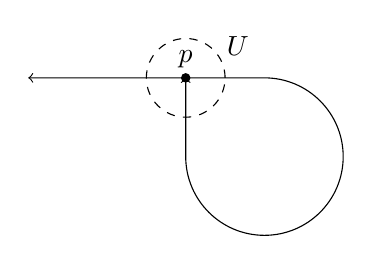
\begin{tikzpicture}[scale=2]
      \coordinate(p) at (0,0);
      \filldraw[black] (p) circle (0.75pt) node[above]{\(p\)};
      \draw[<->] (p) -- ++(0,-0.5) arc (-180:90:0.5) -- (-1,0);
      % \draw[<->] (p) .. controls (0,-1) and (1.5,0) .. (p) -- +(-1,0);
      \draw[dashed] (p) circle (0.25);
      \node[right] (ulabel) at (0.2,0.2) {\(U\)};
    \end{tikzpicture}
    \caption{Ejemplo de inmersión que no forma subvariedad}
    \label{fig:inmersion-no-subvd}
  \end{figure}
\end{example}

\begin{lemma}[label={lem:subvd-diftop}]
  Si \(N\) es subvariedad de \(M\), entonces la \nameref{def:diftop} de la
  estructura de variedad de \(N\) coincide con la topología relativa de la
  \nameref{def:diftop} de \(M\).
\end{lemma}

\begin{proof}
  Sea \(G \subseteq N\) abierto de la \nameref{def:diftop} de \(N\). Sea \(p \in
  G\) y sea \((U,\varphi)\) una carta de \(M\) con \(p \in U\) cumpliendo la
  propiedad de \nameref{def:subvd}. Entonces \(\varphi(G \cap U \cap N)\) es
  abierto de \(\varphi(U \cap N)\) y por tanto \(G \cap U \cap N\) es abierto de
  \(\varphi(U \cap N)\) (que es abierto de la topología relativa de \(N\) pues
  \(U\) es abierto de \(M\)).

  Así, \(G \cap U \cap N\) es abierto de la topología relativa y \(p \in G \cap
  U \cap N \subseteq G\), por lo que \(G\) es abierto de la relativa.

  Ahora sea \(G \subseteq N\) abierto de la topología relativa, i.e. \(G =
  \Omega \cap N\) con \(\Omega\) abierto de la DIF-topología de \(M\).
\end{proof}

\begin{definition}
  Una aplicación diferenciable \(f \colon M \to N\) se dice \emph{incrustación}
  (\emph{embedding}) si es inmersión inyectiva y la DIF-topología de estructura
  diferenciable de \(f(M)\) inducida por \(f \colon M \to f(M)\) coincide con la
  relativa de \(M\)
\end{definition}

\begin{lemma}
  Si \(f \colon M \to N\) es incrustación,
  \begin{enumerate}
  \item \(f(M)\) es subvariedad.
  \item La estructura de subvariedad coincide con la inducida por \(f\).
  \item \(f\) es difeomorfismo.
  \end{enumerate}
\end{lemma}

\end{document}

%%% Local Variables:
%%% TeX-master: "../VD"
%%% End: